\documentclass[11pt]{article}

% ---------- packages ----------
\usepackage[a4paper,margin=1in]{geometry}
\usepackage[T1]{fontenc}
\usepackage[utf8]{inputenc}
\usepackage{amsmath,amssymb,mathtools}
\usepackage{empheq}
\usepackage{graphicx}
\usepackage{booktabs}
\usepackage{xcolor}
\usepackage[most]{tcolorbox}
\usepackage{listings}
\usepackage{caption}
\usepackage{enumitem}
\usepackage[expansion=false]{microtype}
\usepackage[hidelinks]{hyperref}
\usepackage[round,authoryear]{natbib}

% ---------- colors ----------
\definecolor{cint}{HTML}{C0392B}
\definecolor{cbal}{HTML}{27AE60}
\definecolor{cext}{HTML}{2980B9}
\definecolor{srcbg}{HTML}{F4F1EC}
\definecolor{srcbar}{HTML}{8A7A5C}
\definecolor{plainbg}{HTML}{EAF4FB}
\definecolor{plainbar}{HTML}{2980B9}

% ---------- boxes ----------
% Quote from the source paper (provenance)
\newtcolorbox{fromtext}[1]{
  enhanced, breakable, colback=srcbg, colframe=srcbar,
  boxrule=0pt, leftrule=3pt, arc=1pt, left=8pt, right=8pt, top=6pt, bottom=6pt,
  fontupper=\itshape,
  attach title to upper=\quad, coltitle=srcbar, fonttitle=\normalfont\footnotesize\scshape,
  title={From Han \& Gu (2025), #1}}

% Plain-language gloss for the psychologist
\newtcolorbox{plainbox}{
  enhanced, breakable, colback=plainbg, colframe=plainbar,
  boxrule=0pt, leftrule=3pt, arc=1pt, left=8pt, right=8pt, top=6pt, bottom=6pt,
  coltitle=plainbar, fonttitle=\bfseries\footnotesize\scshape,
  title={In plain words}}

% ---------- code ----------
\lstset{
  basicstyle=\ttfamily\scriptsize, breaklines=true, columns=fullflexible,
  keywordstyle=\color{cext}, commentstyle=\color{cbal}\itshape,
  stringstyle=\color{cint}, showstringspaces=false, frame=single,
  rulecolor=\color{gray!40}, language=Python, numbers=left, numberstyle=\tiny\color{gray}}

\newcommand{\sig}{\sigma}
\newcommand{\real}{\mathbb{R}}

\title{\vspace{-1.2cm}\textbf{From ``Balance'' to Dynamics}\\[4pt]
\large A Control-Theoretic Formalization of the Metacognitive\\ Balance Perspective of Han \& Gu (2025)}
\author{\textit{Working note, prepared for the collaboration with Prof.\ Mihwa Han}\\[2pt]\small [Your name]}
\date{\today}

\begin{document}
\maketitle
\vspace{-0.6cm}

\begin{abstract}
\noindent Han \& Gu (2025) argue that cognitive and social functioning in schizophrenia is governed less by \emph{the order} in which self-awareness and context/other-awareness are trained than by their \emph{concurrent co-regulation}, and they picture this balance as movement within an ``adaptive corridor'' policed by immediate ``pivots.'' This note takes their verbal framework at face value and asks a narrow question: \emph{if we write these claims down as equations, does the resulting system actually reproduce the clinical phenomena they describe?} I formalize interpretation as a probabilistic belief, metacognition as a control law acting on that belief, and the self--context referencing system as a coupled dial. A minimal single-scenario realization then reproduces, without extra assumptions, four described phenomena: consolidation of a threat belief under over-internalization, erratic cue-tracking under over-externalization, jumping-to-conclusions as premature confidence, and the rescue of a consolidating belief by a within-session pivot. Two further studies show that the chapter's own ``minimal indices'' (confidence--outcome congruence and tolerance of ambiguity) separate the regimes, and that concurrent co-regulation quantitatively outperforms a gated ``self-then-context'' sequence. Every modeling decision is anchored to the specific sentence in \citet{HanEtAL2025} that motivated it, and every mathematical object is glossed in plain language. This is offered as an \emph{interpretation} of the chapter, not a competing theory.
\end{abstract}

% =====================================================================
\section{Purpose, and how to read this note}
\label{sec:purpose}

The balance-oriented perspective of \citet{HanEtAL2025} is stated as a \emph{conceptual} direction; the authors explicitly reserve formalization for later work. This note is a first attempt at that formalization, written so that it can be read from two sides at once. For the modeler, the goal is a system of differential equations that is simple enough to simulate and inspect. For the psychologist---and especially for Prof.\ Han, whose chapter this formalizes---the goal is that each equation be traceable to a sentence she wrote, and that no symbol go unexplained. Wherever an equation appears, a shaded blue box restates it in ordinary language.

\begin{plainbox}
Think of this note as a translation. The chapter is written in the language of clinical observation; I am re-writing the \emph{same claims} in the language of mathematics, the way one might re-score a piece of music for a different instrument. The tune should be recognizably yours. If any box does not sound like what you meant, that is exactly the kind of mismatch worth catching early.
\end{plainbox}

\paragraph{Notation at a glance.} A handful of symbols recur. Table~\ref{tab:notation} lists them in plain terms.

\begin{table}[h]
\centering\small
\caption{The symbols used in this note, in ordinary language.}
\label{tab:notation}
\begin{tabular}{@{}l l p{7.7cm}@{}}
\toprule
Symbol & Reads as & Plain meaning\\
\midrule
$L(t)$ & ``log-odds of threat'' & a single number for the belief: $0$ = truly unsure (50/50), positive = leaning ``it's about me / threatening,'' negative = ``benign.''\\
$\sig(L)$ & ``sigmoid of $L$'' & an S-shaped squashing function turning $L$ into a probability in $[0,1]$.\\
$b(t)=\sig(L)$ & ``belief'' & the probability the person currently assigns to the threat reading.\\
$\alpha(t)$ & ``self-weight'' & a dial in $[0,1]$: how much inner signals count vs.\ outer cues.\\
$\dfrac{dL}{dt}$ & ``rate of change of $L$'' & how fast the belief is moving \emph{right now}.\\
$\kappa$ & ``leak'' & a gentle pull back toward ``not sure yet'' (guards over-commitment).\\
$\gamma,\ \alpha_0$ & ``gain, set-point'' & how strongly, and toward what habitual lean, the dial returns.\\
$u(t)$ & ``control input'' & the therapist's nudge (a pivot / micro-cycle).\\
\bottomrule
\end{tabular}
\end{table}

% =====================================================================
\section{From the text to the equations}
\label{sec:model}

I build the model in the order the chapter builds its argument: first what a metacognitive judgment \emph{is}, then that it is \emph{controlled}, then that the control has a \emph{self--context dial}, and finally what happens when the dial is stuck or is nudged.

% ---------------------------------------------------------------
\subsection{Interpretation is a probability, not a verdict}

\begin{fromtext}{p.~1}
\dots the capacity to consistently integrate and interpret thoughts, feelings, and bodily sensations in light of others' intentions, prevailing social norms, and situational cues, and to regulate responses accordingly.
\end{fromtext}

\noindent Two things are asserted here. First, a metacognitive output is an \emph{interpretation} formed by \emph{integrating} internal material (thoughts, feelings, sensations) with external material (others' intentions, norms, cues). Second, that interpretation feeds \emph{regulation}. I therefore split the construct into an output (the interpretation) and a controller (the regulation), and I make the output a \emph{probability} rather than a fixed answer, because the chapter repeatedly treats premature certainty as pathological:

\begin{fromtext}{p.~5}
Decisions are often driven by automatic feelings (``feeling = fact'') without explicit reflection, leading to premature closure (JTC) before controlled re-appraisal comes online.
\end{fromtext}

\noindent For a single ambiguous social event with two readings---$h_1$ (benign) and $h_2$ (threat / self-referential)---I represent the interpretation as the posterior probability of the threat reading, written on the log-odds scale:
\begin{equation}
L(t) \;=\; \log\frac{P(h_2\mid \text{evidence up to }t)}{P(h_1\mid \text{evidence up to }t)},
\qquad
b(t)\;=\;\sig\!\big(L(t)\big)\;=\;\frac{1}{1+e^{-L(t)}} .
\label{eq:belief}
\end{equation}
The \emph{decision} the person acts on is the more probable reading, $\hat h = h_2$ if $b>\tfrac12$ else $h_1$; ``jumping to conclusions'' is then simply committing to $\hat h$ while confidence is high but accumulated evidence is small.

\begin{plainbox}
$L$ is one number that stores the whole belief, and it is deliberately \emph{not} a yes/no. $L=0$ means genuinely undecided; the further from $0$, the more sure. Writing the belief this way lets each new piece of evidence just \emph{add} to $L$, and it makes ``jumping to conclusions'' precise: it is $L$ shooting far from $0$ after very little has actually been added.
\end{plainbox}

% ---------------------------------------------------------------
\subsection{Metacognition is control, so belief obeys a rate law}

\begin{fromtext}{p.~3}
\dots its core is control---i.e., stop, check, and strategy shift.
\end{fromtext}

\noindent If the essence of metacognition is \emph{control} exercised in real time, then the belief is not computed once but continuously steered. This is exactly what a differential equation expresses: it says how the belief \emph{changes each moment} as a function of the current belief and the incoming situation $S(t)$,
\begin{equation}
\frac{dL}{dt} \;=\; \mathcal{M}\big(L(t),\,S(t)\big),
\qquad\text{so that}\qquad
L(t) \;=\; L(0) + \int_{0}^{t}\mathcal{M}\big(L(\tau),S(\tau)\big)\,d\tau .
\label{eq:control}
\end{equation}
The chapter also tells us what the controller \emph{listens to}: Proust's procedural signals.

\begin{fromtext}{p.~2}
\dots monitors and corrects ongoing cognitive processing via metacognitive feelings such as confidence, fluency, and effort.
\end{fromtext}

\noindent I take confidence to be the readable procedural signal, and define it as distance from the undecided point,
\begin{equation}
c(t) \;=\; \big|\,2\,b(t)-1\,\big| \;\in\;[0,1].
\label{eq:conf}
\end{equation}

\begin{plainbox}
Equation~\eqref{eq:control} is just: ``the belief now = the belief a moment ago + the small push metacognition applied.'' Adding up all those small pushes over time is the integral. Nothing here assumes the pushes are large or fast; that is decided by the ingredients we plug into $\mathcal{M}$ next. Confidence \eqref{eq:conf} is $0$ when unsure and $1$ when certain either way.
\end{plainbox}

% ---------------------------------------------------------------
\subsection{The self--context dial (the cognitive referencing system)}

\begin{fromtext}{p.~7}
\dots a cognitive referencing system that tilts toward either an internal (self-reflective) or an external (context/other-oriented) anchor is prone to systematic distortions\dots a dynamic regulator moving between two axes---self-awareness and context/other-awareness---to enable early detection and adjustment of imbalances.
\end{fromtext}

\noindent This sentence gives the model its central moving part. Evidence arrives on two channels, and the controller \emph{weights} them. Let $\alpha(t)\in[0,1]$ be the weight on the internal channel (so $1-\alpha$ is the weight on the external channel; on the simplex these are the two coordinates $\alpha_{\text{self}},\alpha_{\text{context}}$ that you wrote, but one number suffices). The two channels are:
\begin{align}
\text{internal (affect / introspection):}\quad & \lambda_S(L) \;=\; a_S + r\,\sig(L),\\
\text{external (situational cues):}\quad & \lambda_C(t) \;=\; a_C + \xi(t),
\end{align}
where $a_S\ge 0$ is a baseline threat-leaning affect, $a_C\le 0$ says cues tend to \emph{dis}confirm the threat reading, and $\xi(t)$ is time-correlated noise standing for the ambiguity of real situations. The term $r\,\sig(L)$ is the crucial one and is justified in \S\ref{sec:overint}.

\begin{plainbox}
$\alpha$ is a volume knob between two inputs: your own gut/affect on one side, the room's cues on the other. Turn it up and inner feelings dominate the belief; turn it down and outside cues do. The chapter's ``tilt'' \emph{is} this knob sitting off-center.
\end{plainbox}

% ---------------------------------------------------------------
\subsection{Concurrency: a coupled system, not a staircase}

\begin{fromtext}{abstract / p.~2}
\dots a dynamic regulatory capacity that coordinates both axes concurrently and interactively, preventing drifts toward over-internalization \dots and over-externalization.
\end{fromtext}

\noindent Because the two axes are \emph{co-regulated} rather than sequenced, belief and dial evolve \emph{together}. Combining the weighted channels with the leak of \S\ref{sec:purpose}, and letting the dial relax toward a personal set-point while being nudged by the therapist, gives the coupled pair that is the whole model:
\begin{empheq}[box=\fbox]{align}
\frac{dL}{dt}     &= \underbrace{\alpha\,\lambda_S(L)}_{\text{self}} \;+\; \underbrace{(1-\alpha)\,\lambda_C(t)}_{\text{context}} \;-\; \kappa L,
\label{eq:sysL}\\[4pt]
\frac{d\alpha}{dt} &= -\,\gamma\,(\alpha-\alpha_0) \;+\; u(t).
\label{eq:sysA}
\end{empheq}
The leak $-\kappa L$ implements the chapter's ``controlled re-appraisal'' and its notion of \emph{calibration} (footnote~1, p.~3: adjusting judgment so confidence tracks evidence): absent fresh evidence, the belief drifts back toward equipoise. (Note: in your draft both lines of the coupled system were typeset as $dX/dt$; the second is the dial's equation, $d\alpha/dt$, as above.)

\begin{plainbox}
Read \eqref{eq:sysL} left to right: the belief is pushed by inner signals \emph{times the knob}, plus outer cues \emph{times one-minus-the-knob}, minus a small pull back toward ``unsure.'' Read \eqref{eq:sysA}: the knob drifts back to the person's habitual setting $\alpha_0$, except when a therapist nudge $u$ moves it. Both happen at the same time---that is the ``concurrent'' in your abstract.
\end{plainbox}

% ---------------------------------------------------------------
\subsection{Over-internalization is a positive-feedback loop}
\label{sec:overint}

\begin{fromtext}{p.~4--5}
\dots over-internalization (excessive self-focus) appears as amplified rumination and guilt or shame, with a preoccupation with ``finding the cause within,'' thereby blocking corrective input from situational cues\dots\ an instance of calibration failure in metacognitive feelings where fluency is mistaken for validity.
\end{fromtext}

\noindent ``Finding the cause within'' and ``fluency mistaken for validity'' describe a loop: the more one already leans toward the self-referential reading, the more one's own affect is taken as further evidence \emph{for} it. That is precisely the term $r\,\sig(L)$: internal evidence grows with current belief. When the dial $\alpha$ is high, this loop can overwhelm the disconfirming external channel and the leak, and $L$ runs away---a consolidated, cue-insensitive threat belief. This is the mathematical signature of a delusion becoming fixed.

\begin{plainbox}
The dangerous ingredient is $r\,\sig(L)$: ``the surer I already am, the more my feelings confirm it.'' With the knob turned toward the inside, this becomes a snowball---each turn adds to itself---and outside reassurance can no longer get in. Turn the knob back down and the snowball stops, which is exactly what the pivot does below.
\end{plainbox}

% ---------------------------------------------------------------
\subsection{Over-externalization is tracking noisy cues}

\begin{fromtext}{p.~5}
\dots overly drawn to others' expressions or behaviors or to rumors while neglecting internal monitoring\dots\ rendering responses erratic across situations.
\end{fromtext}

\noindent When $\alpha$ is small, \eqref{eq:sysL} is dominated by $(1-\alpha)\,\lambda_C(t)$, i.e.\ by the \emph{noisy} external channel. The belief then follows the moment-to-moment fluctuation of whichever cue is salient---``erratic across situations''---with weak internal anchoring. No separate mechanism is needed; erraticism falls out of a low knob feeding on ambiguous input.

% ---------------------------------------------------------------
\subsection{Pivots and micro-cycles are the control input $u(t)$}

\begin{fromtext}{p.~6, footnote 3}
\dots when imbalance signals---over-internalization or over-externalization---are detected, immediately switches the rule-set between self- and context-work to recenter the trajectory within the adaptive corridor.
\end{fromtext}

\noindent This defines $u(t)$ as \emph{feedback} control: it reads an imbalance signal and pushes the dial the other way. A minimal law, faithful to Pivot~A (over-internalization $\rightarrow$ context-work) and Pivot~B (over-externalization $\rightarrow$ self-work), is
\begin{equation}
u(t)=\left\{
\begin{array}{@{}l@{\quad}l@{\quad}l@{}}
-\,p & \text{if } b>\theta_H \text{ and } \dot L>0 & \text{(Pivot A: consolidating $\Rightarrow$ knob out)}\\[3pt]
+\,p & \text{if } \alpha<\theta_L \text{ and } |\dot b|\text{ large} & \text{(Pivot B: cue-driven $\Rightarrow$ knob in)}\\[3pt]
0 & \text{otherwise} & \text{(inside the corridor: do nothing).}
\end{array}\right.
\label{eq:pivot}
\end{equation}
The 5-step micro-cycle (footnote~2, p.~6) is the repeated application of this loop: rate confidence $\to$ generate alternatives $\to$ weigh evidence $\to$ reweight cues $\to$ recalibrate confidence, on the order of $30$--$180$\,s (p.~9). In the implementation the thresholds are split into engage/release pairs ($\theta_H^{\text{on}}>\theta_H^{\text{off}}$), a hysteresis (Schmitt-trigger) latch that prevents the pivot from chattering at the boundary; \eqref{eq:pivot} shows the logic in its simplest form.

\begin{plainbox}
$u$ is the therapist watching the dial. If the belief is snowballing inward, $u$ turns the knob \emph{outward} (list the room's cues, take a third-person view). If the person is blown about by every cue, $u$ turns it \emph{inward} (separate feeling from thought). When things are balanced, $u$ does nothing---the corridor is where no correction is needed.
\end{plainbox}

% ---------------------------------------------------------------
\subsection{The four control parameters are already in the chapter}

Strikingly, the chapter lists the very parameters this model needs:

\begin{fromtext}{p.~9}
\dots (1) confidence gain---the rate at which confidence rises relative to evidence, (2) ambiguity threshold\dots (3) cue weighting---relative allocation to internal versus external cues, and (4) switch sensitivity---the ease stop-check-shift routines can be invoked.
\end{fromtext}

\noindent Each maps to a knob in \eqref{eq:sysL}--\eqref{eq:pivot} (Table~\ref{tab:params}), which is strong evidence that the formalization is tracking the chapter rather than importing outside structure. The between-session ``baseline tilt (set-point) and regulatory gain'' (p.~8) are $\alpha_0$ and $\gamma$; the alignment with Jung's introversion--extraversion (p.~8) is the observation that $\alpha_0$ is a personality parameter.

\begin{table}[h]
\centering\small
\caption{The chapter's control parameters (p.~9) map one-to-one onto the model.}
\label{tab:params}
\begin{tabular}{@{}lll@{}}
\toprule
Chapter's parameter (p.~9) & Model quantity & Plain meaning\\
\midrule
confidence gain & small $\kappa$ / fast $|L|$ growth & how fast certainty outruns evidence\\
ambiguity threshold & tolerance of $\xi$ before commit & how long you can sit with not-knowing\\
cue weighting & $\alpha$ & inner-vs-outer allocation (the dial)\\
switch sensitivity & pivot gain $p$, thresholds $\theta_H,\theta_L$ & how easily a pivot fires\\
baseline tilt (p.~8) & $\alpha_0$ & the habitual lean (a personality trait)\\
regulatory gain (p.~8) & $\gamma$ & how strongly the dial returns home\\
\bottomrule
\end{tabular}
\end{table}

% =====================================================================
\section{Simulation experiments}
\label{sec:exp}

I now ask whether the system \eqref{eq:belief}--\eqref{eq:pivot} \emph{behaves} as the chapter says people behave. All runs use the single ``they laughed at me'' scenario from the clinical vignette (p.~12); parameters are in Appendix~\ref{app:params}, code in Appendix~\ref{app:code}.

% ----
\subsection{Experiment 1 --- three regimes from one personality set-point}
\textbf{Claim tested (p.~7):} a system that ``tilts toward either an internal\dots or an external\dots anchor is prone to systematic distortions.'' \textbf{Setup:} vary only the set-point $\alpha_0\in\{0.85,0.5,0.15\}$; everything else fixed. \textbf{Result} (Fig.~\ref{fig:exp1}): with $\alpha_0=0.85$ the ruminative loop $r\,\sig(L)$ drives the threat belief to $\approx0.98$ with high confidence, ignoring the disconfirming cue (delusion-like fixity); with $\alpha_0=0.5$ the belief stays near equipoise at low confidence (ambiguity tolerated); with $\alpha_0=0.15$ the belief is low but visibly erratic, tracking cue noise---matching ``responses erratic across situations'' (p.~5). One trait parameter reproduces all three described clinical pictures.

\begin{figure}[h]\centering
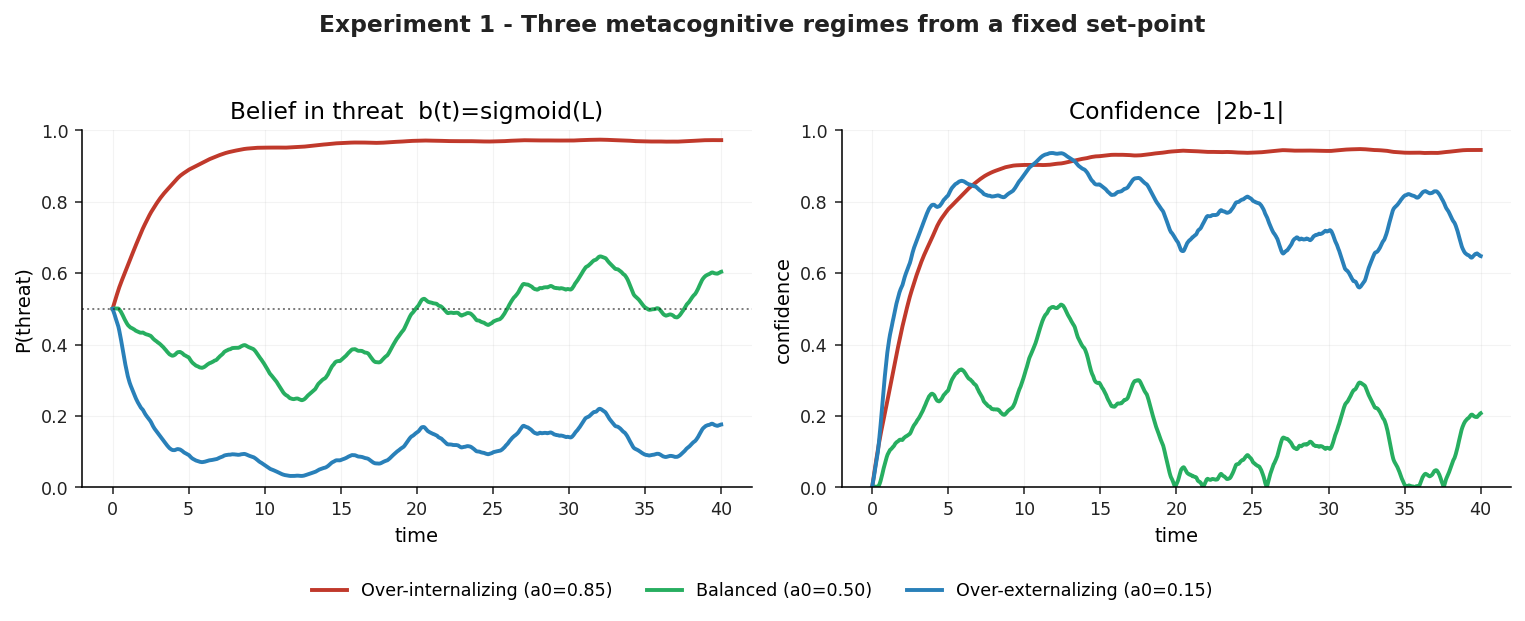
\includegraphics[width=\linewidth]{figs/exp1_regimes.png}
\caption{Belief $b(t)$ and confidence $c(t)$ under the three set-points. Over-internalization consolidates; balance stays uncertain; over-externalization is erratic.}
\label{fig:exp1}
\end{figure}

% ----
\subsection{Experiment 2 --- jumping to conclusions as premature confidence}
\textbf{Claim tested (p.~5):} ``feeling = fact\dots leading to premature closure (JTC).'' \textbf{Setup:} a high-gain configuration (small leak $\kappa$, high $\alpha_0$) vs.\ a cautious one; commitment when $c$ crosses a threshold $c^\ast=0.8$. \textbf{Result} (Fig.~\ref{fig:exp2}): the high-gain agent crosses $c^\ast$ after very little evidence has accumulated, while the cautious agent never over-commits. JTC appears here not as an added rule but as confidence outrunning evidence---i.e.\ a large ``confidence gain'' (p.~9).

\begin{figure}[h]\centering
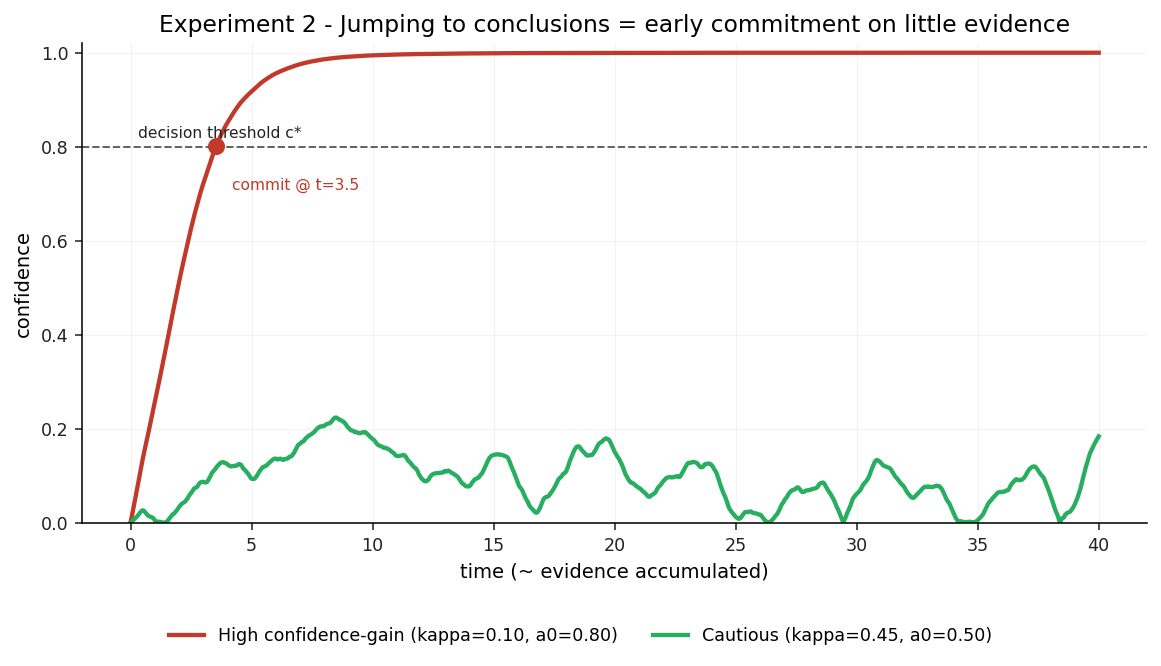
\includegraphics[width=0.82\linewidth]{figs/exp2_jtc.png}
\caption{JTC as early threshold-crossing: high confidence-gain commits on little evidence; the cautious agent stays below the decision line.}
\label{fig:exp2}
\end{figure}

% ----
\subsection{Experiment 3 --- a pivot rescues a consolidating belief}
\textbf{Claim tested (p.~6):} pivots ``recenter the trajectory within the adaptive corridor.'' \textbf{Setup:} the over-internalizing patient of Exp.~1, run with the (hysteretic) pivot law \eqref{eq:pivot} on vs.\ off, same noise seed. \textbf{Result} (Fig.~\ref{fig:exp3}): without intervention the belief locks at $\approx0.97$; with the pivot, once $b$ rises past the engage threshold $\theta_H^{\text{on}}$ the dial $\alpha$ is pushed down, disconfirming cues re-enter, and the belief is pulled back toward the corridor, releasing only when $b$ falls below $\theta_H^{\text{off}}$. The intermittent firing of $\alpha$ is the repeated micro-cycle---the model's picture of \emph{why} the loop must be brief and iterated (p.~5)---while the hysteresis band keeps it from chattering.

\begin{figure}[h]\centering
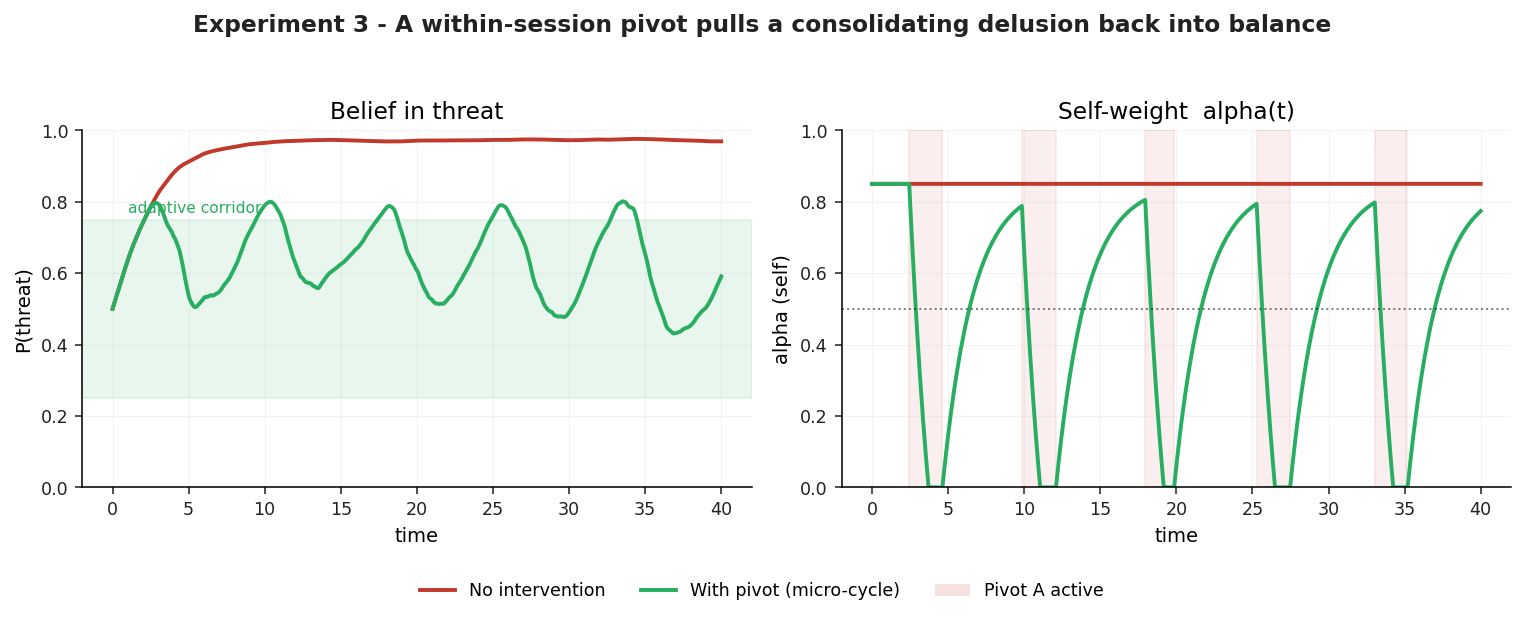
\includegraphics[width=\linewidth]{figs/exp3_pivot.png}
\caption{With vs.\ without the pivot. Left: the intervened belief stays out of consolidation. Right: $\alpha(t)$ shows Pivot~A firing repeatedly (shaded).}
\label{fig:exp3}
\end{figure}

% ----
\subsection{Experiment 4 --- the adaptive corridor as an attractor}
\textbf{Claim tested (p.~7):} ``A diagonal `adaptive corridor' indicates balanced co-regulation, with a pivot to self-work at the upper left and to context-work at the lower right.'' \textbf{Setup:} the self/context engagement plane of your Figure~2, with a vector field that relaxes toward the diagonal and pivots that push out of the two risk corners. \textbf{Result} (Fig.~\ref{fig:exp4}): the corridor becomes a genuine \emph{attractor}---trajectories from both risk corners are drawn back into the band---turning the chapter's static map into dynamics.

\begin{figure}[h]\centering

\includegraphics[width=0.66\linewidth]{figs/exp4_corridor.png}
\caption{The adaptive corridor rendered as a dynamical attractor in the self/context plane (cf.\ Fig.~2 of the chapter).}
\label{fig:exp4}
\end{figure}

% ----
\subsection{Experiment 5 --- the two minimal indices are diagnostic of balance}
\textbf{Claim tested (p.~6):} tracking \emph{confidence--outcome congruence} and \emph{tolerance of ambiguity} suffices to read out balance. \textbf{Setup:} for each regime I run a truth-balanced ensemble (the hidden state is threat or benign with equal probability) and, at commitment, record confidence and correctness; congruence is summarized by the Expected Calibration Error (ECE, the average gap between confidence and accuracy). Separately, I present a genuinely ambiguous stimulus (internal and external evidence cancel, elevated noise) and measure how long the agent stays with it before confidence crosses a commit level. \textbf{Result} (Fig.~\ref{fig:exp5}): the balanced regime is best calibrated (lowest ECE, its reliability curve hugging the diagonal) and the most ambiguity-tolerant; the over-internalizer is confidently wrong (large ECE---the chapter's ``persistent overconfidence $\rightarrow$ suspect internal excess,'' p.~12), and the over-externalizer commits fastest on noise (low tolerance---``jumping-to-conclusions,'' p.~12). The chapter's two low-burden indices thus separate the regimes on their own.

\begin{figure}[h]\centering

\includegraphics[width=\linewidth]{figs/exp5_indices.png}
\caption{The paper's minimal indices. (a) Reliability diagram with ECE per regime; balance is best calibrated. (b) Tolerance of ambiguity; balance stays with not-knowing longest.}
\label{fig:exp5}
\end{figure}

% ----
\subsection{Experiment 6 --- concurrent co-regulation beats a gated sequence}
\textbf{Claim tested (Table~1, p.~4; \S2.4):} concurrent co-regulation should outperform a strict ``self $\rightarrow$ context'' sequence. \textbf{Setup:} on the same substrate and noise, I compare a \emph{sequential} policy (the set-point $\alpha_0(t)$ is gated: high, i.e.\ self-work, for the first half; low, i.e.\ context-work, for the second half; no feedback) against the \emph{balanced} policy (the hysteretic pivot). A burst of threat-consistent evidence is injected mid-run to probe recovery. I score corridor dwell-time (fraction of time the belief stays in the balanced band) and recovery time after the perturbation. \textbf{Result} (Fig.~\ref{fig:exp6}): the balanced policy spends far more time in the corridor (dwell $0.84$ vs.\ $0.12$) and re-enters it faster after the shock (recovery $3.5$ vs.\ $5.9$). A fixed schedule is repeatedly ``in the wrong mode'' for the moment's demand; state-dependent co-regulation is not---exactly the chapter's argument, now quantified.

\begin{figure}[h]\centering
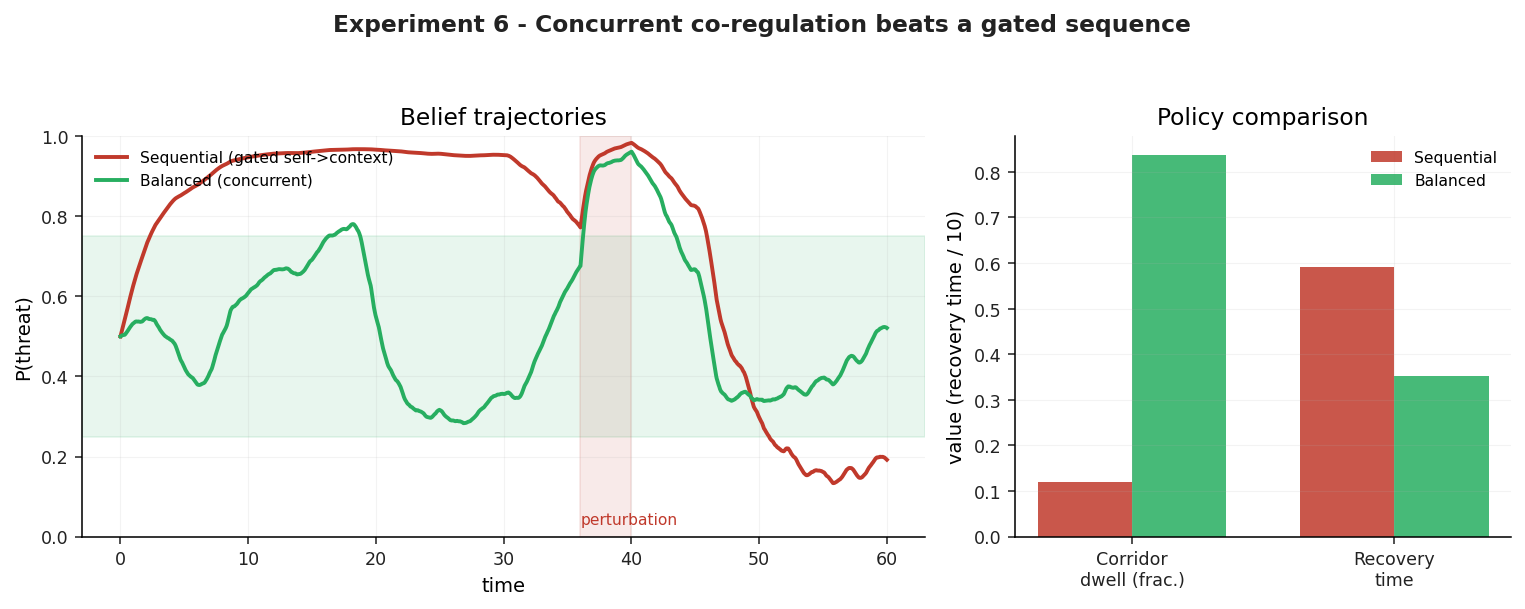
\includegraphics[width=\linewidth]{figs/exp6_policy.png}
\caption{Sequential (gated) vs.\ balanced (concurrent) policy under a mid-run perturbation. Left: belief trajectories with the corridor and perturbation shaded. Right: corridor dwell-fraction and (scaled) recovery time.}
\label{fig:exp6}
\end{figure}

% =====================================================================
\section{Discussion}
\label{sec:disc}

\paragraph{What the formalization buys.} Three of the chapter's claims are, in the model, not assumptions but \emph{consequences}. Over-internalization consolidating into fixity, over-externalization being erratic, and JTC being premature confidence all emerge from the single coupled system once the ruminative feedback term $r\,\sig(L)$ and the dial $\alpha$ are in place. The strongest internal check is Table~\ref{tab:params}: the four control parameters the model requires are the four the chapter already names on p.~9. Experiments~5--6 add quantitative support: the chapter's two minimal indices separate the regimes, and its verbal preference for concurrency over sequence becomes a measurable gap in corridor dwell-time and recovery speed.

\paragraph{Limitations and honest caveats.} This is one scenario with two hypotheses; nothing here speaks to hallucinations or to multi-agent social settings. The pivot law \eqref{eq:pivot} is a caricature of a clinician's judgment. And, as the chapter itself stresses (p.~10, \S4.1), an immediate in-session effect is \emph{not} lasting metacognitive change; the model's fast dynamics should not be over-read as the slow internalization the chapter cares about.

\paragraph{What was refined here, and what remains.} Two refinements flagged in an earlier draft are now in the model. The pivot uses a \emph{hysteresis} band (separate engage/release thresholds $\theta_H^{\text{on}},\theta_H^{\text{off}}$), which removes the chattering seen with a bare threshold and reads as a clinician \emph{committing} to a rebalancing move rather than flickering at the boundary. And interpretation is kept as a posterior while an explicit \emph{commitment} read-out (the $\arg\max$ at decision time) is used to compute the Exp.~5 indices. Remaining work is empirical rather than structural: fitting the parameters of Table~\ref{tab:params} to real confidence--outcome and ambiguity-tolerance logs, and extending beyond a single two-hypothesis scene.

\paragraph{Status.} Following the chapter, this is offered as a conceptual/quantitative \emph{interpretation}, a candidate formal specification of the kind the authors reserved for future work---not a validated model. Its value is as a shared, runnable object we can now poke at together.

% =====================================================================
\appendix
\section{Collected model and parameters}
\label{app:params}
The full system, for reference:
\begin{align*}
\dot L &= \alpha\big(a_S + r\,\sig(L)\big) + (1-\alpha)\big(a_C+\xi(t)\big) - \kappa L, &
\dot\alpha &= -\gamma(\alpha-\alpha_0) + u(t),\\
d\xi &= -\theta\,\xi\,dt + \sigma_C\,dW, &
c &= |2\sig(L)-1|,
\end{align*}
with $u(t)$ from \eqref{eq:pivot}. Baseline parameters:
$a_S=0.20$, $r=1.20$, $a_C=-0.70$, $\sigma_C=0.50$, $\theta=1.0$, $\kappa=0.30$, $\gamma=0.50$, pivot gain $p=0.9$, hysteresis $\theta_H^{\text{on}}=0.78$, $\theta_H^{\text{off}}=0.62$, $\theta_L=0.25$. Set-point $\alpha_0$ is varied per experiment; Exp.~2 uses $\kappa\in\{0.10,0.45\}$. Exp.~5 runs a truth-balanced ensemble (evidence set to favor threat or benign per trial) and an ambiguous stimulus ($a_S=0.40$, $a_C=-0.40$, $\sigma_C=0.70$). Exp.~6 drives $\alpha_0(t)$ as a gated schedule for the sequential policy and injects a threat-evidence burst (magnitude $1.6$ over a short window) to probe recovery.

\section{Reference implementation}
\label{app:code}
Figures are produced by the \texttt{mcbalance} package (\texttt{model.py}, \texttt{metrics.py}, \texttt{experiments.py}); see the project repository for the full source, metrics, and a one-command reproduction script. The reusable core dynamics (explicit Euler--Maruyama, $dt=0.02$, hysteretic pivot latch):
\lstinputlisting{model_listing.py}

\bibliographystyle{plainnat}
\bibliography{references}

\end{document}
